\section{Embedded Linux application development}

\begin{frame}
  \frametitle{Contents}
  \begin{itemize}
  \item Application development
    \begin{itemize}
    \item Developing applications on embedded Linux
    \item Building your applications
    \end{itemize}
  \item Source management
    \begin{itemize}
    \item Integrated development environments (IDEs)
    \item Version control systems
    \end{itemize}
  \item Debugging and analysis tools
    \begin{itemize}
    \item Debuggers
    \item Memory checkers
    \item System analysis
    \end{itemize}
  \end{itemize}
\end{frame}

\subsection{Developing applications on embedded Linux}

\begin{frame}
  \frametitle{Application development}
  \begin{itemize}
  \item An embedded Linux system is just a normal Linux system, with
    usually a smaller selection of components
  \item In terms of application development, developing on embedded
    Linux is exactly the same as developing on a desktop Linux system
  \item All existing skills can be re-used, without any particular
    adaptation
  \item All existing libraries, either third-party or in-house, can be
    integrated into the embedded Linux system
    \begin{itemize}
    \item Taking into account, of course, the limitation of the
      embedded systems in terms of performance, storage and memory
    \end{itemize}
  \item Application development could start on x86, even before
      the hardware is available.
  \end{itemize}
\end{frame}

\begin{frame}
  \frametitle{Programming language (1)}
  \begin{itemize}
  \item The programming language for system-level applications
    in Linux is usually C
    \begin{itemize}
    \item The C library is already present on your system, nothing to
      add
    \end{itemize}
  \item C++ can be used for larger applications
    \begin{itemize}
    \item The C++ library must be added to the system
    \item Some libraries, including Qt, are developed in C++ so they
      need the C++ library on the system anyway
    \end{itemize}
  \item The Rust language is increasingly popular in embedded
      and system applications, as an alternative to C and C++.\\
      See \url{https://www.rust-lang.org/what/embedded}
      for attractive features.
  \item Suggestion to start with Rust if you neither know
      C and C++.
  \end{itemize}
\end{frame}

\begin{frame}
  \frametitle{Programming language (2)}
  \begin{itemize}
  \item Scripting languages can also be useful for quick application
    development, web applications or scripts
    \begin{itemize}
    \item But they require an interpreter on the embedded system and
      have usually higher memory consumption and slightly lower
      performance
    \item Most popular: Python, shell
    \end{itemize}
  \item All programming languages can be used: Lua, Ada, Java, Go...
  \end{itemize}
\end{frame}

\begin{frame}
  \frametitle{C library or higher-level libraries?}
  \begin{itemize}
  \item For many applications, the C library already provides a
    relatively large set of features
    \begin{itemize}
    \item file and device I/O, networking, threads and
      synchronization, inter-process communication
    \item Thoroughly described in the glibc manual, or in any {\em
        Linux system programming} book
    \item However, the API carries a lot of history and is not
      necessarily easy to grasp for new comers
    \end{itemize}
  \item Therefore, using a higher level framework, such as Qt or the
    Gtk/Glib stack, might be a good idea
    \begin{itemize}
    \item These frameworks are not only graphical libraries, their
      core is separate from the graphical part
    \item But of course, these libraries have some memory and storage
      footprint, in the order of a few megabytes
    \end{itemize}
  \end{itemize}
\end{frame}

\begin{frame}
  \frametitle{Building your applications}
  \begin{itemize}
  \item For simple applications that do not need to be really portable
    or provide compile-time configuration options, a simple Makefile
    will be sufficient
  \item For more complicated applications, or if you want to be able
    to run your application on a desktop Linux PC and on the target
    device, using a build system is recommended
    \begin{itemize}
    \item {\em autotools} is ancient, complicated but very
      widely used.
    \item We recommend to invest in simpler and more modern tools
          instead, such as {\em CMake} and {\em Meson}.
    \end{itemize}
  \end{itemize}
\end{frame}

\begin{frame}[fragile]
  \frametitle{Simple Makefile (1)}
  Case of an application that only uses the C library, contains two source
  files and generates a single binary\\
  \includegraphics[height=0.7\textheight]{slides/sysdev-application-development/simple-makefile1.pdf}
\end{frame}

\begin{frame}[fragile]
  \frametitle{Simple Makefile (2)}
  Case of an application that uses the Glib and the GPS libraries\\
  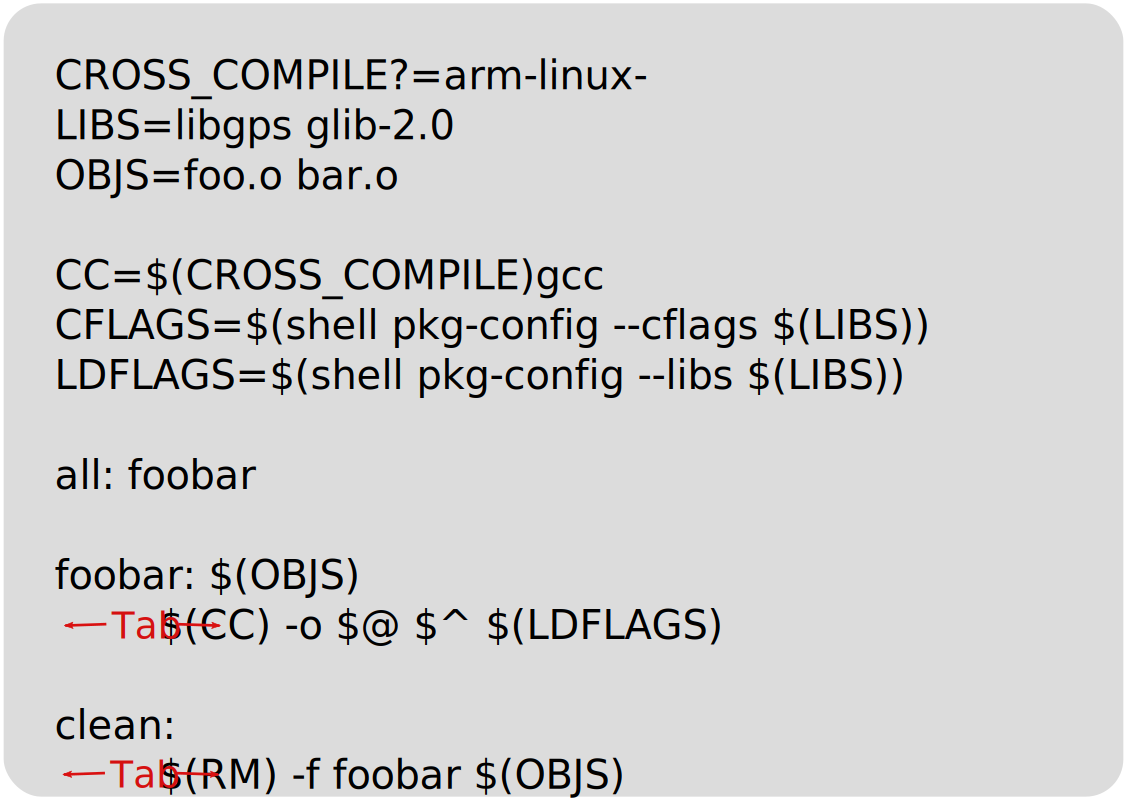
\includegraphics[height=0.7\textheight]{slides/sysdev-application-development/simple-makefile2.pdf}\\
\end{frame}

\subsection[Source management \& IDEs]{Integrated
  Development Environments (IDE)}

\begin{frame}
  \frametitle{Visual Studio Code}
  \begin{columns}
    \column{0.65\textwidth}
    \begin{itemize}
    \item \url{https://code.visualstudio.com/}
    \item Created by Microsoft, MIT licensed
    \item Extensible, language agnostic text editor
    \item Built-in git commands
    \item The most popular IDE (open-source and proprietary) according Stack Overflow's 2019 survey
    \item Try it on Ubuntu:\\
          \code{sudo snap install --classic code}
    \item See Michael Opdenacker's {\em Using Visual Studio Code for Embedded Development} presentation
          (\href{https://bootlin.com/pub/conferences/2020/elce/opdenacker-using-vs-code-for-embedded-development/}{slides},
          \href{https://www.youtube.com/watch?v=YGOZIIOWujc}{video}) at ELCE 2020.
    \end{itemize}
    \column{0.35\textwidth}
    \begin{center}
    \includegraphics[height=0.3\textheight]{slides/sysdev-application-development/visual-studio-code.pdf}\\
    \tiny Image credits (Wikipedia): \url{https://frama.link/RjFqWGBS}\\
    \vspace{0.5cm}
    \includegraphics[width=\textwidth]{common/opdenacker-using-vscode.jpg}
    \end{center}
  \end{columns}
\end{frame}

\begin{frame}
  \frametitle{Eclipse (1)}
  \begin{columns}[T]
    \column{0.7\textwidth}
    \url{https://www.eclipse.org/}
    \begin{itemize}
    \item An extensible, plug-in based software development kit,
      typically used for creating IDEs.
    \item Supported by the Eclipse Foundation, a non-profit consortium
      of major software industry vendors (IBM, Intel, Borland, Nokia,
      Wind River, Zend, Computer Associates...).
    \item Free Software license (Eclipse Public License). Incompatible
      with the GPL.
    \item Supported platforms: GNU/Linux, UNIX, Windows
    \end{itemize}
    Extremely popular: created a lot of attraction.
    \column{0.3\textwidth}
    
\includegraphics[width=0.9\textwidth]{slides/sysdev-application-development/eclipse.pdf}
    \vspace{1cm}\\
    \tiny Image credits:\\
    \url{https://frama.link/C6FJ7Py5}
  \end{columns}
\end{frame}

\begin{frame}
  \frametitle{Eclipse (2)}
  \begin{itemize}
  \item Eclipse is actually a platform composed of many projects:\\
    \url{https://www.eclipse.org/projects/}
    \begin{itemize}
    \item Some projects are dedicated to integrating into Eclipse
      features useful for embedded developers (cross-compilation,
      remote development, remote debugging, etc.)
    \end{itemize}
  \item The platform is used by major embedded Linux software vendors
    for their (proprietary) system development kits: MontaVista
    DevRocket, TimeSys TimeStorm, Wind River Workbench, Sysgo ELinOS.
  \item Eclipse now supports the Theia project
    (\url{https://theia-ide.org/}) that supports VS Code extensions,
    but with its own architecture. It's now used in many IDEs:
    new Arduino PRO IDE, ARM mbed, Eclipse Che...
  \end{itemize}
\end{frame}

\begin{frame}
  \frametitle{Other popular solutions}
  \begin{columns}[T]
    \column{0.6\textwidth}
    \begin{itemize}
    \item Many embedded Linux developers simply use {\bf Vim} or {\bf
        Emacs}. They can integrate with debuggers, source code browsers
        such as {\em cscope}, offer syntax highlighting and more.
    \item People also use {\bf QtCreator}, even for non Qt projects
    \item {\bf Atom} (from GitHub) is a very popular text editor too
    \item See Stack Overflow's survey of most popular IDEs (2019): \url{https://frama.link/bfPgbb88}
    \end{itemize}
    All these tools are available in most Linux distributions, simply
    install them and try them out!
    \column{0.4\textwidth}
    {\small Vim \\
    \includegraphics[height=0.38\textheight]{slides/sysdev-application-development/vim-screenshot.png}\\
    Emacs \\
    \includegraphics[height=0.38\textheight]{slides/sysdev-application-development/emacs-screenshot.png}
    }
  \end{columns}
\end{frame}

\subsection{Version control systems}

\begin{frame}
  \frametitle{Version control systems}
  Real projects can't do without them
  \begin{itemize}
  \item Allow multiple developers to contribute on the same
    project. Each developer can see the latest changes from the
    others, or choose to stick with older versions of some components.
  \item Allow to keep track of changes, and revert them if needed.
  \item Allow developers to have their own development branch
    (branching)
  \item Supposed to help developers resolving conflicts with different
    branches (merging)
  \end{itemize}
\end{frame}

\begin{frame}
  \frametitle{Traditional version control systems}
  Rely on a central repository. {\bf Subversion} is the {\bf last} popular open-source one:
  \begin{itemize}
  \item \url{https://subversion.apache.org/}
  \item Created as a replacement of the old CVS, removing many of its
      limitations.
  \item Commits on several files, proper renaming support, better
      performance, etc.
  \item The user interface is very similar to CVS
  \item \url{https://en.wikipedia.org/wiki/Subversion_(software)}
  \item Fun: see Linus Torvalds expressing his love for CVS and Subversion:
        \url{https://youtu.be/4XpnKHJAok8}
  \end{itemize}
  No longer recommended for new projects. Use distributed source control
  systems instead!
\end{frame}

\begin{frame}
  \frametitle{Distributed source control systems (1)}
  No longer have a central repository
  \begin{itemize}
  \item More adapted to the way the Free Software community develops
    software and organizes
  \item Allows each developer to have a full local history of the
    project, to create local branches. Makes each developer's work
    easier.
  \item People get working copies from other people's working copies,
    and exchange changes between themselves. Branching and merging is
    made easier.
  \item Make it easier for new developers to join, making their own
    experiments without having to apply for repository access.
  \end{itemize}
\end{frame}

\begin{frame}
  \frametitle{Distributed source control systems (2)}
  \begin{itemize}
  \item {\bf Git}
    \begin{itemize}
    \item Initially designed and developed by Linus Torvalds for Linux
      kernel development
    \item Extremely popular in the community, and used by more and
      more projects (Linux, U-Boot, Barebox, uClibc, GNOME, X.org,
      etc.)
    \item Outstanding performance, in particular in big projects
    \item \url{https://en.wikipedia.org/wiki/Git_(software)}
    \end{itemize}
  \item {\bf Mercurial}
    \begin{itemize}
    \item Another system, created with the same goals as Git.
    \item Used by some big projects too
    \item \url{https://en.wikipedia.org/wiki/Mercurial}
    \end{itemize}
  \end{itemize}
  \url{https://en.wikipedia.org/wiki/Version_control_systems\#Distributed_revision_control}
\end{frame}

\subsection{Debuggers}

\begin{frame}
  \frametitle{GDB}
  \fontsize{11}{11}\selectfont
  \begin{columns}[T]
    \column{0.8\textwidth}
    The {\bf GNU Project Debugger}\\
    \url{https://www.gnu.org/software/gdb/}
    \begin{itemize}
    \item The debugger on GNU/Linux, available for most embedded
      architectures.
    \item Supported languages: C, C++, Pascal, Objective-C, Fortran,
      Ada...
    \item Console interface (useful for remote debugging).
    \item Can also be used through graphical IDEs
    \item Can be used to control the execution of a program, set
      breakpoints or change internal variables. You can also use it to
      see what a program was doing when it crashed (by loading its
      memory image, dumped into a \code{core} file).
    \item New alternative: {\em lldb} (\url{https://lldb.llvm.org/})\\
      from the LLVM project.
    \end{itemize}
    See also \url{https://en.wikipedia.org/wiki/Gdb}
    \column{0.2\textwidth}
    \includegraphics[width=0.9\textwidth]{slides/sysdev-application-development/gdb.png}
  \end{columns}
\end{frame}

\begin{frame}
  \frametitle{GDB crash course (1)}
  \small
  A few useful GDB commands
  \begin{itemize}
  \item \code{break foobar} (\code{b})\\
    Put a breakpoint at the entry of function \code{foobar()}
  \item \code{break foobar.c:42}\\
    Put a breakpoint in \code{foobar.c}, line 42
  \item \code{print var} or \code{print task->files[0].fd} (\code{p})\\
    Print the variable \code{var}, or a more complicated reference. GDB
    can also nicely display structures with all their members
  \end{itemize}
\end{frame}

\begin{frame}
  \frametitle{GDB crash course (2)}
  \small
  \begin{itemize}
  \item \code{continue} (\code{c})\\
    Continue the execution after a breakpoint
  \item \code{next} (\code{n})\\
    Continue to the next line, stepping over function calls
  \item \code{step} (\code{s})\\
    Continue to the next line, entering into subfunctions
  \item \code{backtrace} (\code{bt})\\
    Display the program stack
  \end{itemize}
\end{frame}

\subsection{Remote debugging}

\begin{frame}
  \frametitle{Remote debugging}
  \begin{itemize}
  \item In a non-embedded environment, debugging takes place using \code{gdb}
    or one of its front-ends.
  \item \code{gdb} has direct access to the binary and libraries compiled
    with debugging symbols.
  \item However, in an embedded context, the target platform
    environment is often too limited to allow direct debugging with
    \code{gdb} (2.4 MB on x86).
  \item Remote debugging is preferred
    \begin{itemize}
    \item \code{ARCH-linux-gdb} is used on the development workstation, offering
      all its features.
    \item \code{gdbserver} is used on the target system (only 100 KB
      on arm).
    \end{itemize}
  \end{itemize}
  \begin{center}
    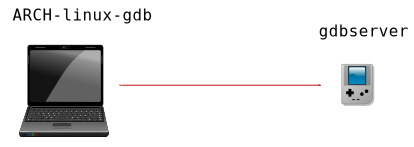
\includegraphics[width=0.5\textwidth]{slides/sysdev-application-development/gdb-vs-gdbserver.pdf}
  \end{center}
\end{frame}

\begin{frame}
  \frametitle{Remote debugging: architecture}
  \begin{center}
    \includegraphics[width=\textwidth]{slides/sysdev-application-development/gdb-vs-gdbserver-architecture.pdf}
  \end{center}
\end{frame}

\begin{frame}
  \frametitle{Remote debugging: usage}
  \begin{itemize}
  \item On the target, run a program through \code{gdbserver}.\\
    Program execution will not start immediately.\\
    \code{gdbserver localhost:<port> <executable> <args>}
    \code{gdbserver /dev/ttyS0 <executable> <args>}
  \item Otherwise, attach \code{gdbserver} to an already running program:\\
    \code{gdbserver --attach localhost:<port> <pid>}
  \item Then, on the host, start \code{ARCH-linux-gdb <executable>},\\
    and use the following \code{gdb} commands:
    \begin{itemize}
    \item To connect to the target:\\
      \code{gdb> target remote <ip-addr>:<port>} (networking)\\
      \code{gdb>  target remote /dev/ttyUSB0} (serial link)
    \item To tell \code{gdb} where shared libraries are:\\
      \code{gdb> set sysroot <library-path>} (without \code{lib/})
    \end{itemize}
  \end{itemize}
\end{frame}

\begin{frame}
  \frametitle{Post mortem analysis}
  \begin{itemize}
  \item When an application crashes due to a {\em segmentation fault}
    and the application was not under control of a debugger, we get no
    information about the crash
  \item Fortunately, Linux can generate a {\em core} file that
    contains the image of the application memory at the moment of the
    crash, and gdb can use this {\em core} file to let us analyze the
    state of the crashed application
  \item On the target
    \begin{itemize}
    \item Use \code{ulimit -c unlimited} in the shell starting the
    application, to enable the generation of a {\em core} file
    when a crash occurs
    \end{itemize}
  \item On the host
    \begin{itemize}
    \item After the crash, transfer the {\em core} file from the target to
      the host, and run
      \code{ARCH-linux-gdb -c core-file application-binary}
    \end{itemize}
  \end{itemize}
\end{frame}

\subsection{Memory checkers}

\begin{frame}
  \frametitle{Valgrind (1)}
  \begin{columns}[T]
    \column{0.8\textwidth}
    \url{https://valgrind.org/}
    \begin{itemize}
    \item GNU GPL Software suite for debugging and profiling programs.
    \item Supported platforms: Linux on x86, x86\_64, arm (armv7 only),
      arm64, mips32, s390, ppc32 and ppc64. Also supported on other
      operating systems (Android, Darwin, Illumos, Solaris...)
    \item Can detect many memory management and threading bugs.
    \item Profiler: provides information helpful to speed up your
      program and reduce its memory usage.
    \item The most popular tool for this usage. Even used by projects
      with hundreds of programmers.
    \end{itemize}
    \column{0.2\textwidth}
    \includegraphics[width=\textwidth]{slides/sysdev-application-development/valgrind1.png}
  \end{columns}
\end{frame}

\begin{frame}
  \frametitle{Valgrind (2)}
  \begin{columns}[T]
    \column{0.8\textwidth}
    \begin{itemize}
    \item Can be used to run any program, without the need to
      recompile it.
    \item Example usage\\
      \code{valgrind --leak-check=yes ls -la}
    \item Works by adding its own instrumentation to your code and
      then running in on its own virtual cpu core.\\
      Significantly slows down execution, but still fine for testing!
    \item More details on \url{https://valgrind.org/info/} and
      \url{https://valgrind.org/docs/manual/coregrind_core.html}
    \item The Valgrind tool suite is easy to add to your root filesystem
          with Buildroot.
    \end{itemize}
    \column{0.2\textwidth}
    \includegraphics[width=\textwidth]{slides/sysdev-application-development/valgrind2.png}
  \end{columns}
\end{frame}

\subsection{System analysis}

\begin{frame}[fragile]{strace}
  \begin{columns}
  \column{0.75\textwidth}
  \small
  System call tracer - \url{https://strace.io}
  \begin{itemize}
  \item Available on all GNU/Linux systems\\
        Can be built by your cross-compiling toolchain generator or by your build system.
  \item Allows to see what any of your processes is doing: accessing files, allocating memory...
        Often sufficient to find simple bugs.
  \item Usage:\\
    \code{strace <command>} (starting a new process)\\
    \code{strace -f <command>} ({\bf f}ollow child processes too)\\
    \code{strace -p <pid>} (tracing an existing process)\\
    \code{strace -c <command>} (time statistics per system call)
    \code{strace -e <expr> <command>} (use {\bf e}xpression for advanced filtering)
  \end{itemize}
  See \href{https://man7.org/linux/man-pages/man1/strace.1.html}{the strace manual} for details.
  \column{0.25\textwidth}
  \includegraphics[height=0.7\textheight]{common/strace-mascot.png}\\
  \tiny Image credits: \url{https://strace.io/}
  \end{columns}
\end{frame}

\begin{frame}[fragile]{strace example output}
  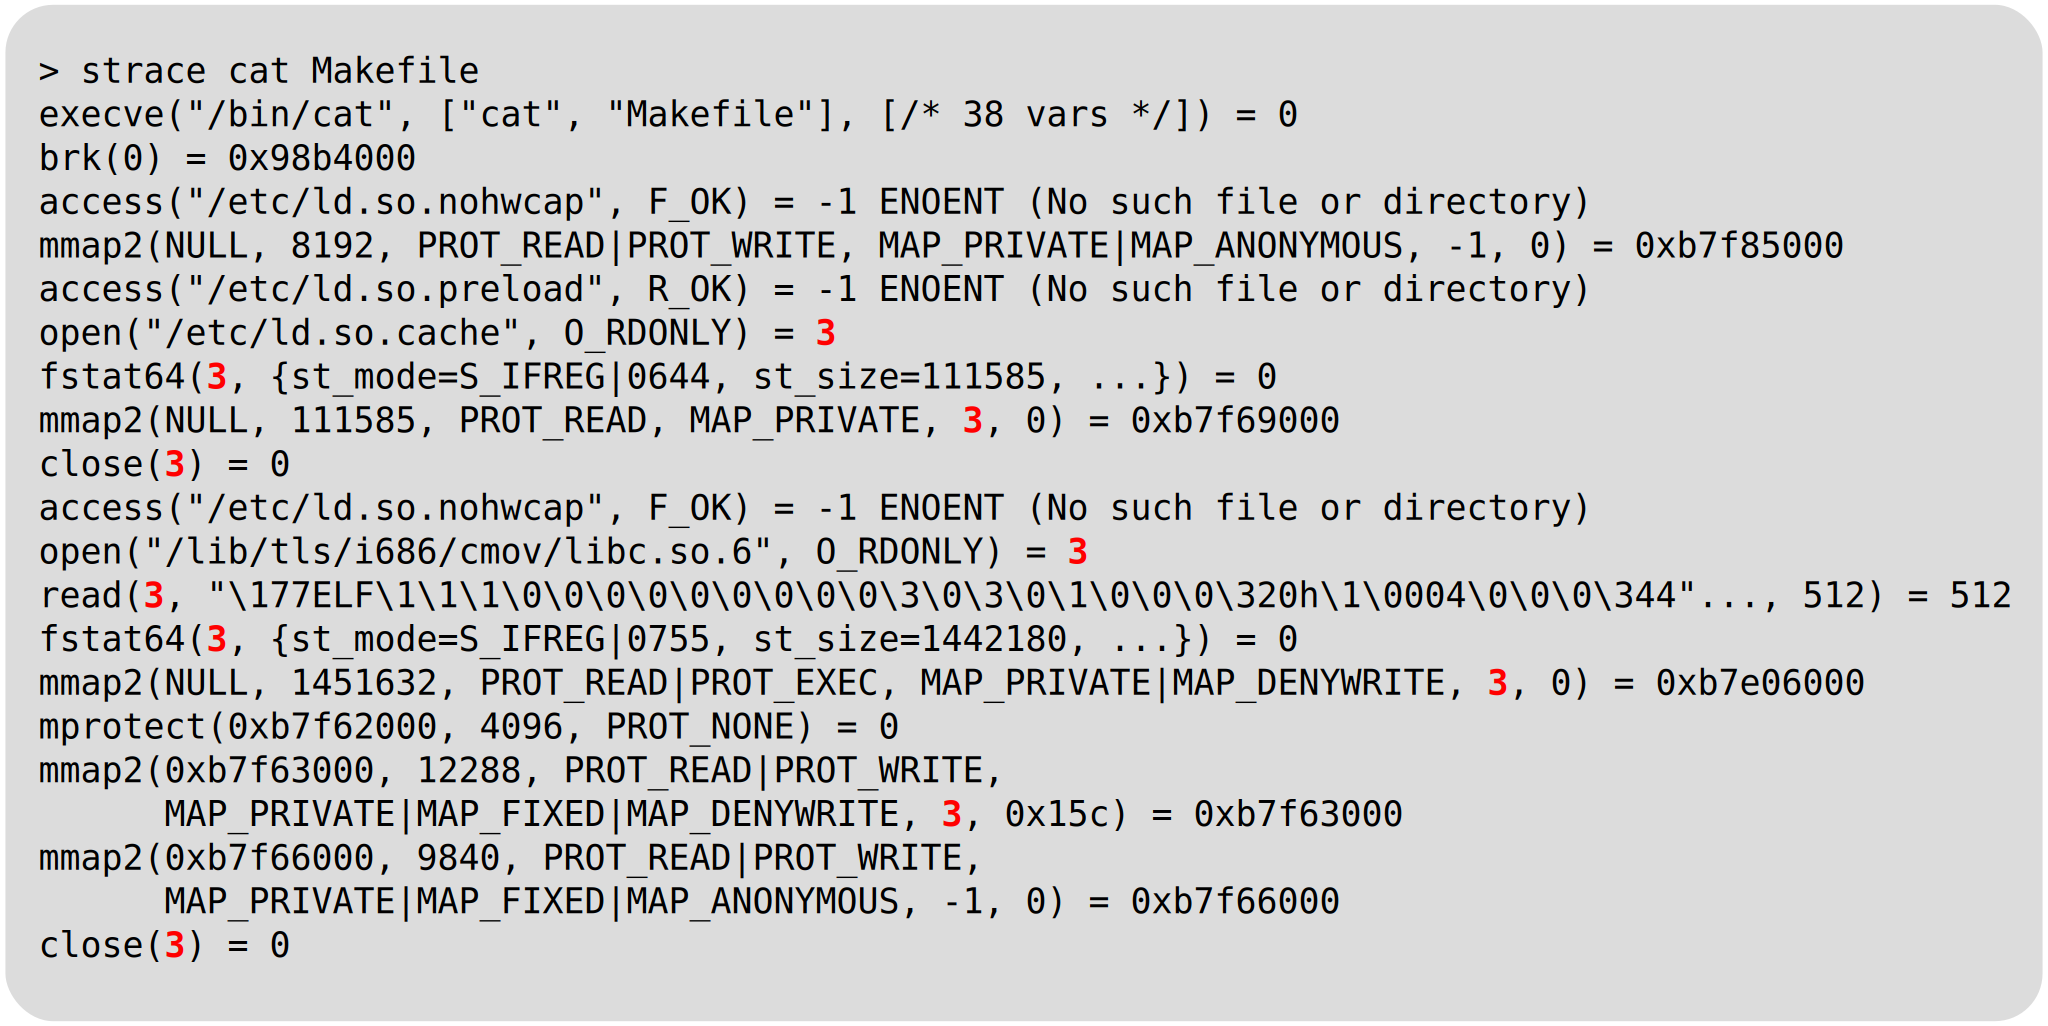
\includegraphics[height=0.75\textheight]{common/strace-output.pdf}\\
  Hint: follow the open file descriptors returned by \code{open()}.
  This tells you what files are handled by further system calls.
\end{frame}

\begin{frame}[fragile]
  \frametitle{strace -c example output}
  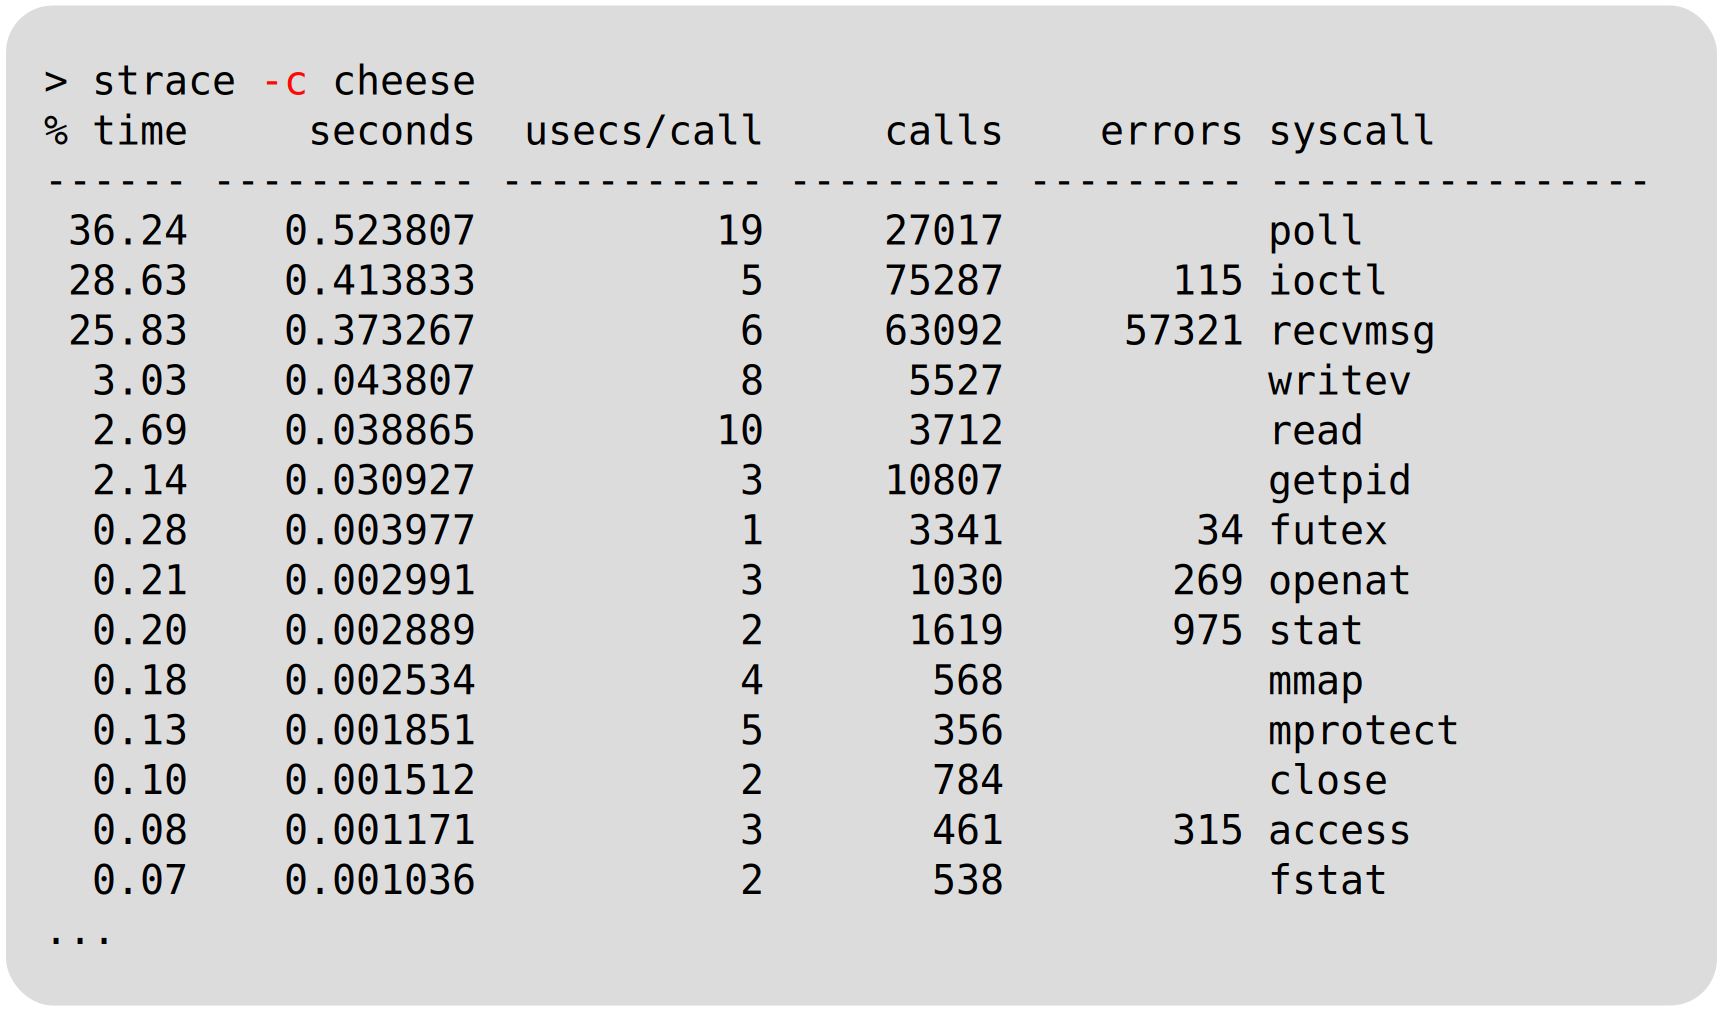
\includegraphics[height=0.8\textheight]{common/strace-c-output.pdf}
\end{frame}

\begin{frame}
  \frametitle{ltrace}
  A tool to trace library calls used by a program and all the signals
  it receives
  \begin{itemize}
  \item Very useful complement to \code{strace}, which shows only system
    calls. Library calls include system calls too!
  \item Of course, works even if you don't have the sources
  \item Allows to filter library calls with regular expressions, or
    just by a list of function names.
  \item Also offers a summary with its \code{-c} option.
  \item Manual page: \url{https://linux.die.net/man/1/ltrace}
  \item Works better with {\em glibc}. \code{ltrace} was broken
        with {\em uClibc} and may still be.
  \end{itemize}
  See \url{https://en.wikipedia.org/wiki/Ltrace} for details
\end{frame}

\begin{frame}[fragile]
  \frametitle{ltrace example output}
  \small
  \begin{block}{}
\begin{verbatim}
ltrace nedit index.html
sscanf(0x8274af1, 0x8132618, 0x8248640, 0xbfaadfe8, 0) = 1
sprintf("const 0", "const %d", 0) = 7
strcmp("startScan", "const 0") = 1
strcmp("ScanDistance", "const 0") = -1
strcmp("const 200", "const 0") = 1
strcmp("$list_dialog_button", "const 0") = -1
strcmp("$shell_cmd_status", "const 0") = -1
strcmp("$read_status", "const 0") = -1
strcmp("$search_end", "const 0") = -1
strcmp("$string_dialog_button", "const 0") = -1
strcmp("$rangeset_list", "const 0") = -1
strcmp("$calltip_ID", "const 0") = -1
\end{verbatim}
\end{block}
\end{frame}


\setuplabframe
{App. development and debugging}
{
  Application development
  \begin{itemize}
  \item Compile your own application with the ncurses library
  \end{itemize}
  Remote debugging
  \begin{itemize}
  \item Set up remote debugging tools on the target:\\
        \code{strace}, \code{ltrace} and \code{gdbserver}.
  \item Debug a simple application running on the target using remote
    debugging
  \end{itemize}
}

